\documentclass[../main.tex]{subfiles}
\begin{document}
\begin{solution}{2}
\subsolution{a}
Använder formel \ref{vecadd}:
\[\vec{u} + \vec{v} = (2, 3) + (1, 5) = (2 + 1, 3 + 5)\]

Bild: 

\begin{center}
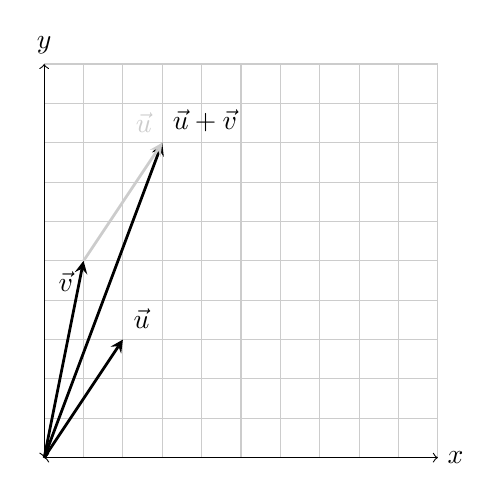
\begin{tikzpicture}[scale=0.5]
  \draw[thin,gray!40] (0,0) grid (10,10);
  \draw[<->] (0,0)--(10,0) node[right]{$x$};
  \draw[<->] (0,0)--(0,10) node[above]{$y$};
  \draw[line width=1pt,-stealth](0,0)--(2,3) node[anchor=south west]{$\vec{u}$};
  \draw[line width=1pt,-stealth](0,0)--(1,5) node[anchor=north east]{$\vec{v}$};
  \draw[line width=1pt,-stealth](0,0)--(3,8) node[anchor=south west]{$\vec{u} + \vec{v}$};
  \draw[line width=1pt,gray!40,-stealth](1,5)--(3,8) node[anchor=south east]{$\vec{u}$};
\end{tikzpicture}
\end{center}

\subsolution{b}
Använder först formel \ref{vecscale}:
\[\vec{u} - \vec{v} = \vec{u} + (-1)\cdot\vec{v} = 
(2, 3) + (-1, -5)\]

Nu är det lätt att använda formel \ref{vecadd}:
\[\vec{u} + \vec{v} = (2, 3) + (-1, -5) = (1, -2)\]

Det här var en övertydlig lösning, enklare skulle vara att bara göra såhär direkt:
\[\vec{u} - \vec{v} = (2 - 1, 3 - 5) = (1, -2)\]

Bild: 

\begin{center}
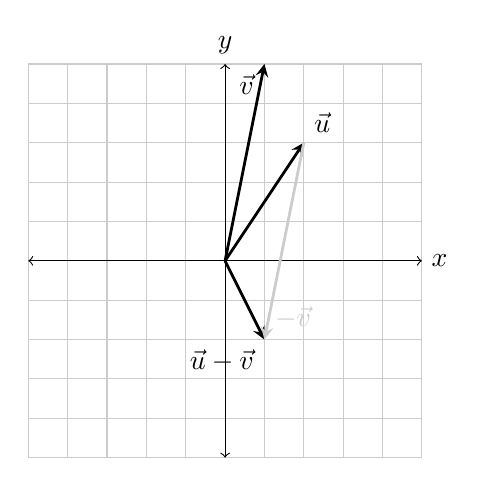
\begin{tikzpicture}[scale=0.5]
  \draw[thin,gray!40] (-5,-5) grid (5,5);
  \draw[<->] (-5,0)--(5,0) node[right]{$x$};
  \draw[<->] (0,-5)--(0,5) node[above]{$y$};
  \draw[line width=1pt,-stealth](0,0)--(2,3) node[anchor=south west]{$\vec{u}$};
  \draw[line width=1pt,-stealth](0,0)--(1,5) node[anchor=north east]{$\vec{v}$};
  \draw[line width=1pt,-stealth](0,0)--(1,-2) node[anchor=north east]{$\vec{u} - \vec{v}$};
  \draw[line width=1pt,gray!40,-stealth](2,3)--(1,-2) node[anchor=south west]{$-\vec{v}$};
\end{tikzpicture}
\end{center}

\subsolution{c}
Använder formel \ref{vecscale}:
\[-2\vec{u} = (-2\cdot 2, -2\cdot 3) = (-4, -6)\]

\begin{center}
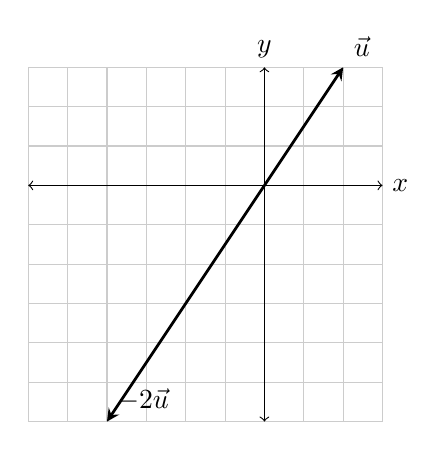
\begin{tikzpicture}[scale=0.5]
  \draw[thin,gray!40] (-6,-6) grid (3,3);
  \draw[<->] (-6,0)--(3,0) node[right]{$x$};
  \draw[<->] (0,-6)--(0,3) node[above]{$y$};
  \draw[line width=1pt,-stealth](0,0)--(2,3) node[anchor=south west]{$\vec{u}$};
  \draw[line width=1pt,-stealth](0,0)--(-4,-6) node[anchor=south west]{$-2\vec{u}$};
\end{tikzpicture}
\end{center}

\end{solution}
\end{document}